%
% LaTeX Problem Set Template by Sachin Padmanabhan
% I created this when I was a freshman in CS 103,
% and I continue to use it to this day.
%
% Hope you enjoy!
%
% There may be problems with this template.
% If so, feel free to contact me.
%

\documentclass{article}
\usepackage{amsmath}
\usepackage{amssymb}
\usepackage{amsthm}
\usepackage{amssymb}
\usepackage{mathdots}
\usepackage[pdftex]{graphicx}
\usepackage{fancyhdr}
\usepackage[margin=1in]{geometry}
\usepackage{multicol}
\usepackage{bm}
\usepackage{listings}
\PassOptionsToPackage{usenames,dvipsnames}{color}  %% Allow color names
\usepackage{pdfpages}
\usepackage{algpseudocode}
\usepackage{tikz}
\usepackage{enumitem}
\usepackage[T1]{fontenc}
\usepackage{inconsolata}
\usepackage{framed}
\usepackage{wasysym}
\usepackage[thinlines]{easytable}
\usepackage{hyperref}
\usepackage{dsfont}

\usepackage{graphicx}
\graphicspath{ {images/} }

\hypersetup{
    colorlinks=true,
    linkcolor=blue,
    filecolor=magenta,
    urlcolor=blue,
}

\title{
\textsc{Iran university of science and technology} \\ [25pt] % Your university, school and/or department name(s)
Discrete mathematics\\Problem Set \#1 \\
}
\author{Ali Heydari}
\date{\today}

\lhead{Ali Heydari}
\chead{Problem Set \#1}
\rhead{\today}
\lfoot{}
\cfoot{Discrete mathematics --- Winter 2018}
\rfoot{\thepage}

\newcommand{\abs}[1]{\lvert #1 \rvert}
\newcommand{\absfit}[1]{\left\lvert #1 \right\rvert}
\newcommand{\norm}[1]{\left\lVert #1 \right\rVert}
\newcommand{\eval}[3]{\left[#1\right]_{#2}^{#3}}
\renewcommand{\(}{\left(}
\renewcommand{\)}{\right)}
\newcommand{\floor}[1]{\left\lfloor#1\right\rfloor}
\newcommand{\ceil}[1]{\left\lceil#1\right\rceil}
\newcommand{\pd}[1]{\frac{\partial}{\partial #1}}
\newcommand{\inner}[1]{\langle#1\rangle}
\newcommand{\cond}{\bigg|}
\newcommand{\rank}[1]{\mathbf{rank}(#1)}
\newcommand{\range}[1]{\mathbf{range}(#1)}
\newcommand{\nullsp}[1]{\mathbf{null}(#1)}
\newcommand{\repr}[1]{\left\langle#1\right\rangle}

\DeclareMathOperator{\Var}{Var}
\DeclareMathOperator{\tr}{tr}
\DeclareMathOperator{\Tr}{\mathbf{Tr}}
\DeclareMathOperator{\diag}{\mathbf{diag}}
\DeclareMathOperator{\dist}{\mathbf{dist}}
\DeclareMathOperator{\prob}{\mathbf{prob}}
\DeclareMathOperator{\dom}{\mathbf{dom}}
\DeclareMathOperator{\E}{\mathbf{E}}
\DeclareMathOperator{\R}{\mathbb{R}}
\DeclareMathOperator{\var}{\mathbf{var}}
\DeclareMathOperator{\quartile}{\mathbf{quartile}}
\DeclareMathOperator{\conv}{\mathbf{conv}}
\DeclareMathOperator{\VC}{VC}
\DeclareMathOperator*{\argmax}{arg\,max}
\DeclareMathOperator*{\argmin}{arg\,min}
\DeclareMathOperator{\Ber}{Bernoulli}
\DeclareMathOperator{\NP}{\mathbf{NP}}
\DeclareMathOperator{\coNP}{\mathbf{coNP}}
\DeclareMathOperator{\TIME}{\mathsf{TIME}}
\DeclareMathOperator{\polytime}{\mathbf{P}}
\DeclareMathOperator{\PH}{\mathbf{PH}}
\DeclareMathOperator{\SIZE}{\mathbf{SIZE}}
\DeclareMathOperator{\ATIME}{\mathbf{ATIME}}
\DeclareMathOperator{\SPACE}{\mathbf{SPACE}}
\DeclareMathOperator{\ASPACE}{\mathbf{ASPACE}}
\DeclareMathOperator{\NSPACE}{\mathbf{NSPACE}}
\DeclareMathOperator{\Z}{\mathbb{Z}}
\DeclareMathOperator{\N}{\mathbb{N}}
\DeclareMathOperator{\EXP}{\mathbf{EXP}}
\DeclareMathOperator{\NEXP}{\mathbf{NEXP}}
\DeclareMathOperator{\NTIME}{\mathbf{NTIME}}
\DeclareMathOperator{\DTIME}{\mathbf{DTIME}}
\DeclareMathOperator{\poly}{poly}
\DeclareMathOperator{\BPP}{\mathbf{BPP}}
\DeclareMathOperator{\ZPP}{\mathbf{ZPP}}
\DeclareMathOperator{\RP}{\mathbf{RP}}
\DeclareMathOperator{\coRP}{\mathbf{coRP}}
\DeclareMathOperator{\BPL}{\mathbf{BPL}}
\DeclareMathOperator{\IP}{\mathbf{IP}}
\DeclareMathOperator{\PSPACE}{\mathbf{PSPACE}}
\DeclareMathOperator{\NPSPACE}{\mathbf{NPSPACE}}
\DeclareMathOperator{\SAT}{\mathsf{SAT}}
\DeclareMathOperator{\NL}{\mathbf{NL}}
\DeclareMathOperator{\PCP}{\mathbf{PCP}}
\DeclareMathOperator{\PP}{\mathbf{PP}}
\DeclareMathOperator{\cost}{cost}
\let\Pr\relax
\DeclareMathOperator*{\Pr}{\mathbf{Pr}}

\definecolor{shadecolor}{gray}{0.95}

\theoremstyle{plain}
\newtheorem*{lem}{Lemma}

\theoremstyle{plain}
\newtheorem*{claim}{Claim}

\theoremstyle{definition}
\newtheorem*{answer}{Answer}

\newtheorem{theorem}{Theorem}[section]
\newtheorem*{thm}{Theorem}
\newtheorem{corollary}{Corollary}[theorem]
\newtheorem{lemma}[theorem]{Lemma}

\renewcommand{\headrulewidth}{0.4pt}
\renewcommand{\footrulewidth}{0.4pt}

\setlength{\parindent}{0pt}

\pagestyle{fancy}

\renewcommand{\thefootnote}{\fnsymbol{footnote}}

\begin{document}

\maketitle

\section{Two Is Irrational?}

In lecture, we proved that $\sqrt{2}$ is irrational, and in the checkpoint problem you proved that $\sqrt{3}$ is irrational.
Below is a purported proof that $\sqrt{4}$ is irrational:

\begin{theorem}
  $\sqrt{4}$  is irrational.
\end{theorem}
\begin{proof}
  Assume for the sake of contradiction that $\sqrt{4}$ is rational. Then there must exist
integers $p$ and $q$ where $ q \neq 0 $, where $p / q = \sqrt{4}$ , and where $p$ and $q$ have no
common factors other than $1$ and$ -1$.
Since $p / q = \sqrt{4}$ , we have $p^2 / q^2 = 4$, so $p^2 = 4q^2$. Since $q^2$ is an integer, we see
that $p^2$ is a multiple of four, and therefore $p$ is a multiple of four. Thus $p = 4n$
for some integer $n$.
Since $4q^2 = p^2$ and $p = 4n$, we have $4q^2 = (4n)^2 = 16n^2$, so $q^2 = 4n^2$. Since $n^2$ is an
integer, we see that $q^2$ is a multiple of four, so $q$ is a multiple of four as well.
But since both $p$ and $q$ are multiples of four, we see that $p$ and $q$ share a common
divisor other than $1$ and $-1$, contradicting our initial assumption. We have
reached a contradiction, so our assumption must have been incorrect. Thus $\sqrt{4}$
is irrational.
\end{proof}
This proof has to be wrong, because$ \sqrt{4} = 2 = 2/1$, which is indeed rational!
What error does this proof make that lets it conclude $\sqrt{4}$ is irrational? Why doesn't this error occur
in the similar proofs that $\sqrt{2}$ and $\sqrt{3}$ are irrational?
\begin{shaded}
\begin{answer}
Just because $p^2$ is divisible by $4$, that doesn't mean $p$ is.
\end{answer}
\end{shaded}

\section{Modular Arithmetic}
Many different numbers yield the same remainder when divided by some number. For example, the
numbers $2, 5, 8, 11, 14$, and $17$, all leave a remainder of two when divided by three, while the numbers
$1, 12, 23, 34,$ and $45$ all leave a remainder of one when divided by eleven. To formalize this relationship
between numbers, we'll introduce a relation $ \equiv_k $  that, intuitively, indicates that two numbers
leave the same remainder when divided by $k$. For example, we'd say that $1 \equiv_{11} 12 $ and that $8 \equiv_3 11$.

\begin{enumerate}[label*=\roman*.,ref=\roman*]
\item Prove that for any integer $x$ and any integer $x$ that $ x \equiv_k x $.
\begin{shaded}
\begin{answer}
\begin{proof}
 $$ \forall x \in \mathds{Z} \quad : \quad k | x - x \quad \Rightarrow \quad x \equiv_k x $$
\end{proof}
\end{answer}
\end{shaded}

\item Prove that for any integers $x$ and $y$ and any integer $k$ that if $x \equiv_k y$, then $y \equiv_k x$.
\begin{shaded}
\begin{answer}
\begin{proof}
$$ \forall x , y \in \mathds{Z} $$
\begin{equation}\label{x , y mod k}
x \equiv_k y \quad \Rightarrow \quad k | x - y
\end{equation}
\begin{equation}\label{x - y = y - x}
  k | x - y \quad = \quad k | y - x
\end{equation}
$$ \text{from} \quad \ref{x - y = y - x}, \ref{x , y mod k} \quad \Rightarrow \quad y \equiv_k x $$
\end{proof}
\end{answer}
\end{shaded}

\item Prove that for any integers $x, y$, and $z$ and any integer $k$ that if $x \equiv_k y$ and $y \equiv_k z$, then $x \equiv_k z$.
\begin{shaded}
\begin{answer}
\begin{proof}
$$ \forall x , y , x \in \mathds{Z} $$
\begin{equation}\label{y , z mod k}
  y \equiv_k z \quad \Rightarrow \quad k | y - z
\end{equation}
$$ \text{from} \quad \ref{x , y mod k} , \ref{y , z mod k} \quad \Rightarrow \quad k | x - z \quad \Rightarrow x \equiv_k z  $$
\end{proof}
\end{answer}
\end{shaded}


\end{enumerate}
\section{Pigeonhole Principle }
\paragraph*{
There are 51 senators in a senate. The senate needs to be divided into $n$ committees such that each senator is on exactly one committee. Each senator hates exactly three other senators.(If senator $A$ hates senator $B$, then senator $B$ does $’not'$ necessarily hate senator $A$.)
}
\paragraph*{
Find the smallest $n$ such that it is always possible to arrange the committees so that no senator hates another senator on his or her committee.
}
\begin{shaded}
\begin{answer}
\begin{proof}
In the worst case, consider that senator $S$ hates a set of 3 senators, while he himself is hated by a completely different set of 3 other senators. Thus, given one senator, there may be a maximum of 6 other senators whom he cannot work with. If we have a minimum of 7 committees, there should be at least one committee suitable for the senator $S$ after the assignment of the 6 conflicting senators.
\end{proof}
\end{answer}
\end{shaded}

\section{Case proof}

\begin{shaded}
\begin{answer}
\begin{proof}
  $$ C - (A\cap B)  \, = \, C \cap (A \cap B)' \, = \, C \cap ( A' \cup B' ) \,
  = \, (C \cap A' ) \cup (C \cap B' ) \, = \, ( C - A ) \cup ( C - B )  $$
\end{proof}
\end{answer}
\end{shaded}

\section{$n \times n$ chessboard}
Consider an $ n \times n $ chessboard with the four corners removed. For which values of $n$ can you cover the board with L- tetrominoes as in Figure. \ref{fig1}?
\begin{figure}[h]
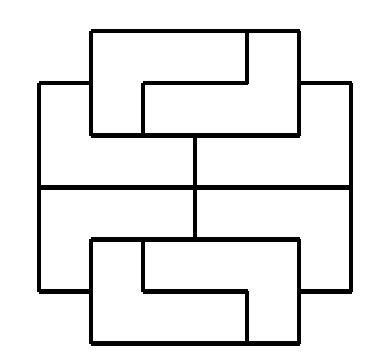
\includegraphics[scale=0.5]{fig1}
\caption{}
\label{fig1}
\end{figure}
\begin{shaded}
\begin{answer}
\begin{proof}
There are $ n^2 — 4 $squares on the board. To cover it with tetrominoes $ n^2 — 4 $ must be a multiple of 4, i.c., n must be even. But this is not sufficient. To sec this, we color the board as in Figure. \ref{fig2} An L-tetromino covers three white and one black squares or three black and one white squares. Since there is an equal number of black and white squares on the board, any complete covering uses an equal number of tetrominoes of each kind. Hence, it uses an even number of tetrominoes, that is, $n^2 — 4$ must be a multiple of 8. So, n must have the form $4k + 2$. By actual construction, it is easy to sec that the condition $4k + 2$ is also sufficient.
\end{proof}
\end{answer}
\end{shaded}
\begin{figure}[h]
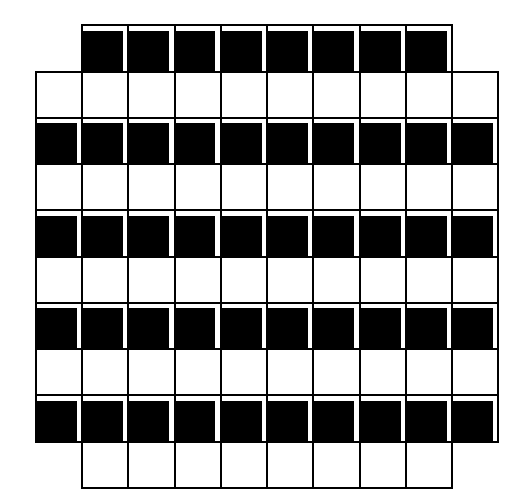
\includegraphics[scale=0.35]{fig2}
\caption{}
\label{fig2}
\end{figure}

\section{Properties of Sets}

Here are some claims about properties of sets. Some of them are true and some of them are false. For each true statement, write a proof that the statement is true. For each false statement, write a \textit{\textbf{disproof}} of the statement (take a look at the Proofwriting Checklist for information about how to write a disproof.) You can use any proof techniques you'd like.
\begin{enumerate}[label*=\roman*.,ref=\roman*]

\item Prove or disprove: for all sets $A$, $B$, and $C$,
if $A \in B$ and $B \in C$, then $A \in C$.

\textit{\textcolor{blue}{ This is your first example of a ``prove or disprove'' problem.
Part of the challenge of approaching a problem like this one is that you'll need to figure out whether or not the statement is even true in the first place, since if it's true you'll want to prove it and if it's false you'll want to disprove it. }}

\textit{\textcolor{blue}{ Here are two strategies for approaching problems like these.
First, try out a lot of examples! You'll want to
get a feel for what the symbolic expression above ``feels'' like in practice. Second, get a sheet of scratch paper
and write out both the statement and its negation. One of those statements is true, and your task is to
figure out which one it is. Once you have those two statements, think about what you would need to do to
prove each of them. In each case, what would you be assuming? What would you need to prove? If you
can answer those questions, you can explore both options and seeing which one ends up panning out. }}

\begin{shaded}
\begin{proof}[Disproof]
$$ A =\{1\} \quad , \quad B=\{\{1\},2\} \quad , \quad  C = \{\{\{1\},2\} , 3\} $$
$$ A \in B \quad \text{and} \quad B \in C \quad \text{But} \quad A \not \in C \qquad \text{\textreferencemark}  $$

\end{proof}
\end{shaded}

\item Prove or disprove: for all sets $A$, $B$, and $C$, if $A \subseteq B$ and $A \subseteq C$, then $A \subseteq B \cap C$.

\begin{shaded}
\begin{proof}
\begin{equation}\label{equ1}
 \text{if} \quad A \subseteq B \quad \Rightarrow \quad \forall x \in A \quad \Rightarrow \quad x \in B
\end{equation}
\begin{equation}\label{equ2}
\text{if} \quad A \subseteq C \quad \Rightarrow \quad \forall x \in A \quad \Rightarrow \quad x \in C
\end{equation}
$\\$
 $$\qquad \ref{equ1} , \ref{equ2} \quad \Rightarrow \forall x \in A \quad \Rightarrow (x \in B) \wedge (x \in C) \quad \Rightarrow \quad A \subseteq (B \cap C) $$

\end{proof}
\end{shaded}

\item Prove or disprove: for all sets $A$, $B$, and $C$, if $A \subsetneq B$ and $A \subsetneq C$, then $A \subsetneq B \cap C$. (The notation $A \subsetneq B$ says that $A$ is a \textit{\textbf{strict subset}} of $B$, meaning that $A \subseteq B$ and $A \neq B$.)

\begin{shaded}
\begin{proof}
  $$ \text{if} \quad A \subseteq (B \cap C) \quad \Rightarrow \quad (A \subseteq B) \wedge (A \subseteq C) \qquad \text{\textreferencemark} $$
\end{proof}
\end{shaded}

\item Prove or disprove: there exists a set $A$ where $\wp(A) = \{A\}$.

\begin{shaded}
-
\end{shaded}

\item Prove or disprove: for all sets $A$ and $B$,
if $\wp(A) = \wp(B)$, then $A = B$.

\textit{\textcolor{blue}{ Look back at Wednesday's lecture. What's a good general way to prove that two sets are equal? }}

\begin{shaded}
\begin{proof}
 $ A = \{1\} \quad B = \{2\} \\
  \Rightarrow \wp(A) = \{ 1, \{1\}\} \quad , \quad \wp(B) = \{ 2, \{2\}\} \quad \text{But} \quad A \neq B \qquad \text{\textreferencemark}$
\end{proof}
\end{shaded}

\end{enumerate}

\textit{\textcolor{blue}{ Before you turn in these proofs, be sure to read over the Proofwriting Checklist and to go one item at a
time through each of your proofs. Here are a few specific things to look for:
\begin{itemize}
\item Make sure that the structures of your proofs match the definitions of the relevant terms. For example,
to prove that a set $S$ is a subset of a set $T$, follow the pattern from lecture: pick an arbitrary
$x \in S$, then prove that $x \in T$ by making specific claims about $x$.
\item However, avoid restating definitions in the abstract. For example, rather than writing
\begin{center}
``We know that $S \subseteq T$ if every element of $S$ is an element of $T$. \\
Therefore, since we know that $A \subseteq B$ and $x \in A$, we see that $x \in B$.''
\end{center}
instead remove that first sentence and just write something like this:
\begin{center}
``Since $x \in A$ and $A \subseteq B$, we see that $x \in B$.''
\end{center}
Whoever is reading your proof knows all the relevant definitions. They're more interested in seeing
\textbf{how those definitions interact with one another} than \textbf{what those definitions are}.
\item Make sure you clearly indicate what each variable means and whether it's chosen arbitrarily or
chosen to have a specific value. For example, in your answers, if you refer to variables like A, B,
or C, you should clearly indicate whether they?re chosen arbitrarily or refer to specific values.
\item If you're talking about an arbitrary set A, it's often tempting to try to list of the elements of A by
writing something like $A = \{ x_1, x_2, \ldots, x_n \}$. The problem with this approach is that by writing
$A = \{ x_1, x_2, \ldots, x_n \}$, you're implicitly saying that the set $A$ is finite, since you're claiming it only
has $n$ elements in it. This is a problem if $A$ is an infinite set. In fact, if $A$ is infinite, because of
Cantor's theorem you can't necessarily even write $A = \{ x_1, x_2, x_3, \ldots \}$, since you might run out of
natural numbers with which to name the elements of $A$ without having listed all of them!
\end{itemize}
}}

\end{document} 